\section{Background}\label{intro-background}

Computer based simulations find numerous applications in medicine. Such applications include training of medical personell, diagnosing patients based on digital data and scientific research to gain better understanding of physiological phenomena. Bio-mechanical simuations are one of the most challenging uses of computer based simulation in medicine. The underlying principles are very complex and thus require sophisticated theoretical formulations and considerable software development efforts.

One of the areas where bio-mechanical simulations are very important is obstetrics related medical simulations.

The main focus of this project is creating a realistic real-time computer based simuation of human childbirth. Simulations of this kind require modeling biomechanical interactions of high complexity. As mentioned, this implyies highly sophisticated. This report will therefore attempt to cover the important aspects of human childbirth.

\section{Human labour}
\subsection{Cardinal movements}
Investigating the mechanisms of labour is an important preliminary step before designing childbirth simulation software. The process of childbirth is complex and involves a multitude of different mechanical processes. \citet{GABBE91} describes the cardinal movements as the main mechanisms of labour and lists seven distinct movements: engagement, descent, flexion, internal rotation, extension, external rotation (restitution) and expulsion. \citet{NORMALLABOUR} gives the following definitions to the movements and provides figures:

\begin{enumerate}
\item Engagement –- this step is identified by the passage of the widest diameter of the fetal skull through the pelvic inlet (Fig \ref{engagementFig}).


\begin{figure}
\begin{minipage}[t]{6cm}
\begin{center}
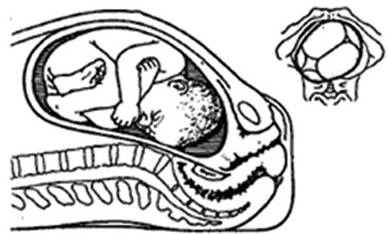
\includegraphics[width=65mm]{sections/introduction/images/Justengagement.png}
\caption{\label{engagementFig} Engagement}
\end{center}
\end{minipage}
\hfill
\begin{minipage}[t]{6cm}
\begin{center}
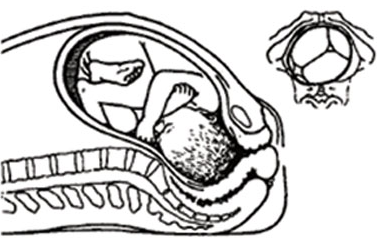
\includegraphics[width=65mm]{sections/introduction/images/Engagementflexion.png}
\caption[Descent and flexion]{\label{flexionFIg} Descent and flexion}
\end{center}
\end{minipage}
\end{figure}


\begin{figure}
\begin{minipage}[t]{6cm}
\begin{center}
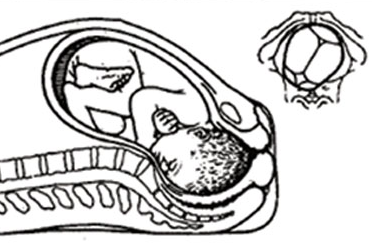
\includegraphics[width=65mm]{sections/introduction/images/InternalRotation.png}
\caption{\label{intRotFig} Internal rotation}
\end{center}
\end{minipage}
\hfill
\begin{minipage}[t]{6cm}
\begin{center}
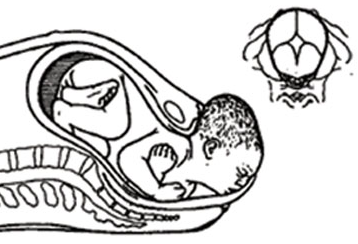
\includegraphics[width=65mm]{sections/introduction/images/Completeextension.png}
\caption[Descent and flexion]{\label{Descent} Extension}
\end{center}
\end{minipage}
\end{figure}

\begin{figure}
\begin{minipage}[t]{6cm}
\begin{center}
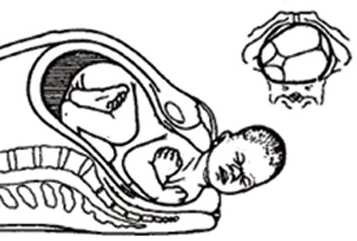
\includegraphics[width=65mm]{sections/introduction/images/ExternalRotation.png}
\caption{\label{ExternalRotationFig} External rotation}
\end{center}
\end{minipage}
\hfill
\begin{minipage}[t]{6cm}
\begin{center}
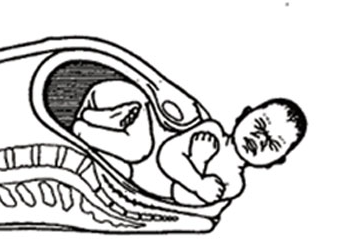
\includegraphics[width=65mm]{sections/introduction/images/Expulsion.png}
\caption[Descent and flexion]{\label{ExpulsionFig} Expulsion}
\end{center}
\end{minipage}
\end{figure}


\item Descent -- the stage when the fetal head passes further downwards through the cervix towards the birth canal (Fig \ref{Descent}).
\item Flexion –- is the process when the fetal head flexes with its chin approaching its chest. The shape of the pelvis and the pelvic floor are said to cause flexion. Flexion allows the fetus to pass through the birth canal with a smaller diameter (e.g. the bi-parietal diameter (Fig \ref{diameters}) (Fig \ref{flexionFIg}).

\begin{figure}
\centering
  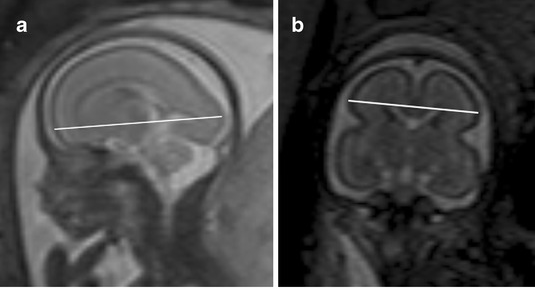
\includegraphics[width=80mm]{sections/introduction/images/DIAMETERS.png}
\caption{ \label{diameters} Fetal head diameters: a -- Fronto-occipital diameter, b -- Cerebral biparietal diameter \citep{DIAMETERS}. }
\end{figure}

\item Internal rotation – is also thought to be caused by the shape of the pelvic canal and soft tissues. It is represented by rotation of the fetal head from facing sideways to facing backwards relative to the mother's body. This can be explained by the fact that the pelvic inlet has the widest diameter in the sideways direction, whereas the pelvic outlet is widest in the sagittal axis (Fig \ref{intRotFig}).

\item Extension –- happens while the neck of the baby is under the pubic symphysis. During extension the head deflexes and in this stage, chin and head are born facing outwards (Fig \ref{Descent}).
\item External rotation (restitution) is represented by external rotation of the head to face sideways as compared to the rest of the body (Fig \ref{ExternalRotationFig}).

\item Expulsion -– when external rotation is complete and the shoulder has moved under the pubic symphysis the fetus is born (Fig \ref{ExpulsionFig}).

\end{enumerate}



\subsection{Problematic labour}

\subsection{Childbirth simulators}
There are a number of mechanical childbirth simulators that exist already. Such simualtors are designed to allow tranee obstetricians and midwifes to interact with a maniquin of a birthing woman. The maniquin is normally made of plastic and/or metal. The section

The motivation behind using a computer based simulation in childbirth modeling is dictated by a number of reasons. While having certain advantages the mechanical childbirth simulators often lack very important features. Primarily, mechanical maniquin will typically be very poorly customizable. Such simulator is typically used for training juniour personnel and in many of training cases the simulation scenario is required to be changed based on the type of the case that is being practiced. Using mechanical simulator means that only a specific scenario is available for training with only slight variations. Additional maniquins of a different type will have to be acquired to perform training for alternative scenarios. Contrary to this, computer based simulations allow unrestricted customizability. It is also worth mentioning, that there exsits a hybrid type of simulators, that combine a computer based underlying bio-mechanical model with an external mechanical maniquin to provide the interface between the trainee and the simulator. Such, simualtors combine the advantages of both types of simulators, but also carry the drawbacks of at least one of them.

Computer simulations provide a good tool for representing real world phenomena, but they are only capable of representing the simulated objects to a certain degree of approximation. Better approximations are predominantly much more expensive in terms of computational power. With the increased processing power of modern computers, it is possible to perform simuations with a higher degree of fidelity. However, even the most performant machines can struggle with certain types of high-cost simulations. In such cases, we have to utilize the underlying hardware to the highest degree possible. This can be achieved by a number optimization techniques. One of the most effective techniques is using parallel processing in order to speed up the computation.

\section{Reverse vs Forward engineered approaches}

There is a number mong the existing mechanical and computer based simulators of human childbirth. It is crucially important to contrast the approach chosen for this research project from the existing reverse-engineered simulations.

\section{Finite element method in surgical simulations}

Finite element method (FEM) is

It is desired to achieve the highest fidelity of the simulaitons with as little latency as possible. To this end, performance optimizations and GPU utilization for Finite Element Analysis is one of the main focuses of this thesis. Several available application programming interfaces (API's) will be overviewed as the candidate tools for implementation. It is then shown how the chosen API is used to achieve highly efficient implementation of FEA for soft-tissue simulation.

Another important aspect of creating a computer based simulation of childbirth is acquiring realistic 3D models of the underlying physiological structures. Namely, the fetal body and maternal lower body geometries are required. The possible ways of constructing the required meshes will be covered in this thesis. The approach is not yet decided on.

\section{Report overview}

The organization of the remainder of this report is presented here.

In chapter \ref{chap-literature} a literature review is conducted  presenting the body of already existing relevant research. The review is split based on relevance to a particular aspect of this research project.

Chapter \ref{chap-methodology} describes the work that has already been undertaken as of the date of this report.

Three publications have been successfully made in the duration of this PhD course, each of which covered an important topic related to the area of interest of this research. All three papers will be covered in this report. The papers are include in the \ref{appendix}.

There is a considerable amount of work still left to complete. The \ref{chap-future} chapter focuses on describing the required steps aimed at achieving the objectives of this research project. An approximate work plan is also presented in this chapter featuring a Gannt chart.

Finally chapter \ref{chap-thesis} presents a proposed thesis structure for the final write-up.
